\question[15] Todas las mañanas Montse y Ricardo se desplazan de sus casas a la escuela.
A ella le gusta caminar y Ricardo utiliza su bicicleta.
En la gráfica de la figura \ref{fig:dist_tiempo_02} se representan sus movimientos.  \par

{\InsertBoxR{0}{
        \parbox[t]{0.5\linewidth}{
            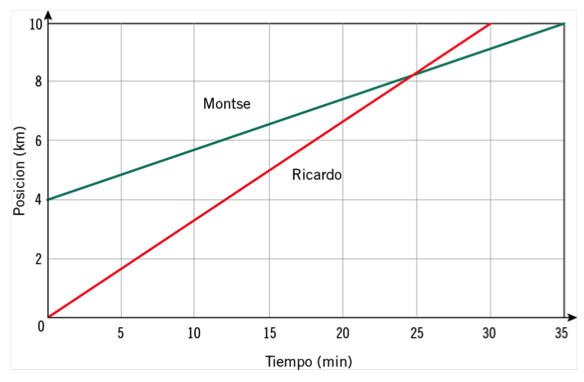
\includegraphics[width=\linewidth]{Images/dist_tiempo_02}
            \captionof{figure}{La gráfica representa los viajes de Montse y Ricardo desde sus casa a la escuela.}
            \label{fig:dist_tiempo_02}
        }
    }}
\hspace{0.5cm}
\begin{parts}
    \begin{minipage}[t]{0.4\linewidth}
        % \subfile{Questions/Parts/question006c}
        \subfile{Questions/Parts/question006d}
        % \subfile{Questions/Parts/question006a}
        \subfile{Questions/Parts/question006b}
        \subfile{Questions/Parts/question006f}
    \end{minipage}
    % \subfile{Questions/Parts/question006e}
    \subfile{Questions/Parts/question006g}
    \subfile{Questions/Parts/question006h}
\end{parts}
